\section{Related Work}
The literature on object detection is vast.
Here we briefly summarize work relevant to our contribution.

An early success in efficient object detection used simple Haar features to build up a \emph{cascade} of classifiers, which then considered image regions in a sliding window regime~\cite{Viola2001}.
Plentiful later work improved the behavior of the cascade while maintaining the basic idea~\cite{Bourdev2005}. \note{more refs}
This detection method is fast, but the simple features and classifiers used have not led to the best performing detectors.

The best performance has recently come from detectors that use gradient-based features to represent either local patches or object-sized windows; if local patches are used, it appears important to include additional feature channels such as shape and color; if object-sized windows are used, finer-scale ``parts'' in object representation boost performance significantly.

%!TEX root=related_work.tex
\begin{figure}[htb]
  \caption{Most object detection approaches have three parts: region proposal, region evaluation, and post-processing of detections. The parts are in a sense sequential, which leads to the influence of cues like context being deferred to the post-processing stage, and to a dependency of early detections on the goodness of proposals. We present a system that considers region proposal and evaluation jointly, such that it is able to output the best detections early in the process.}
  \centering
    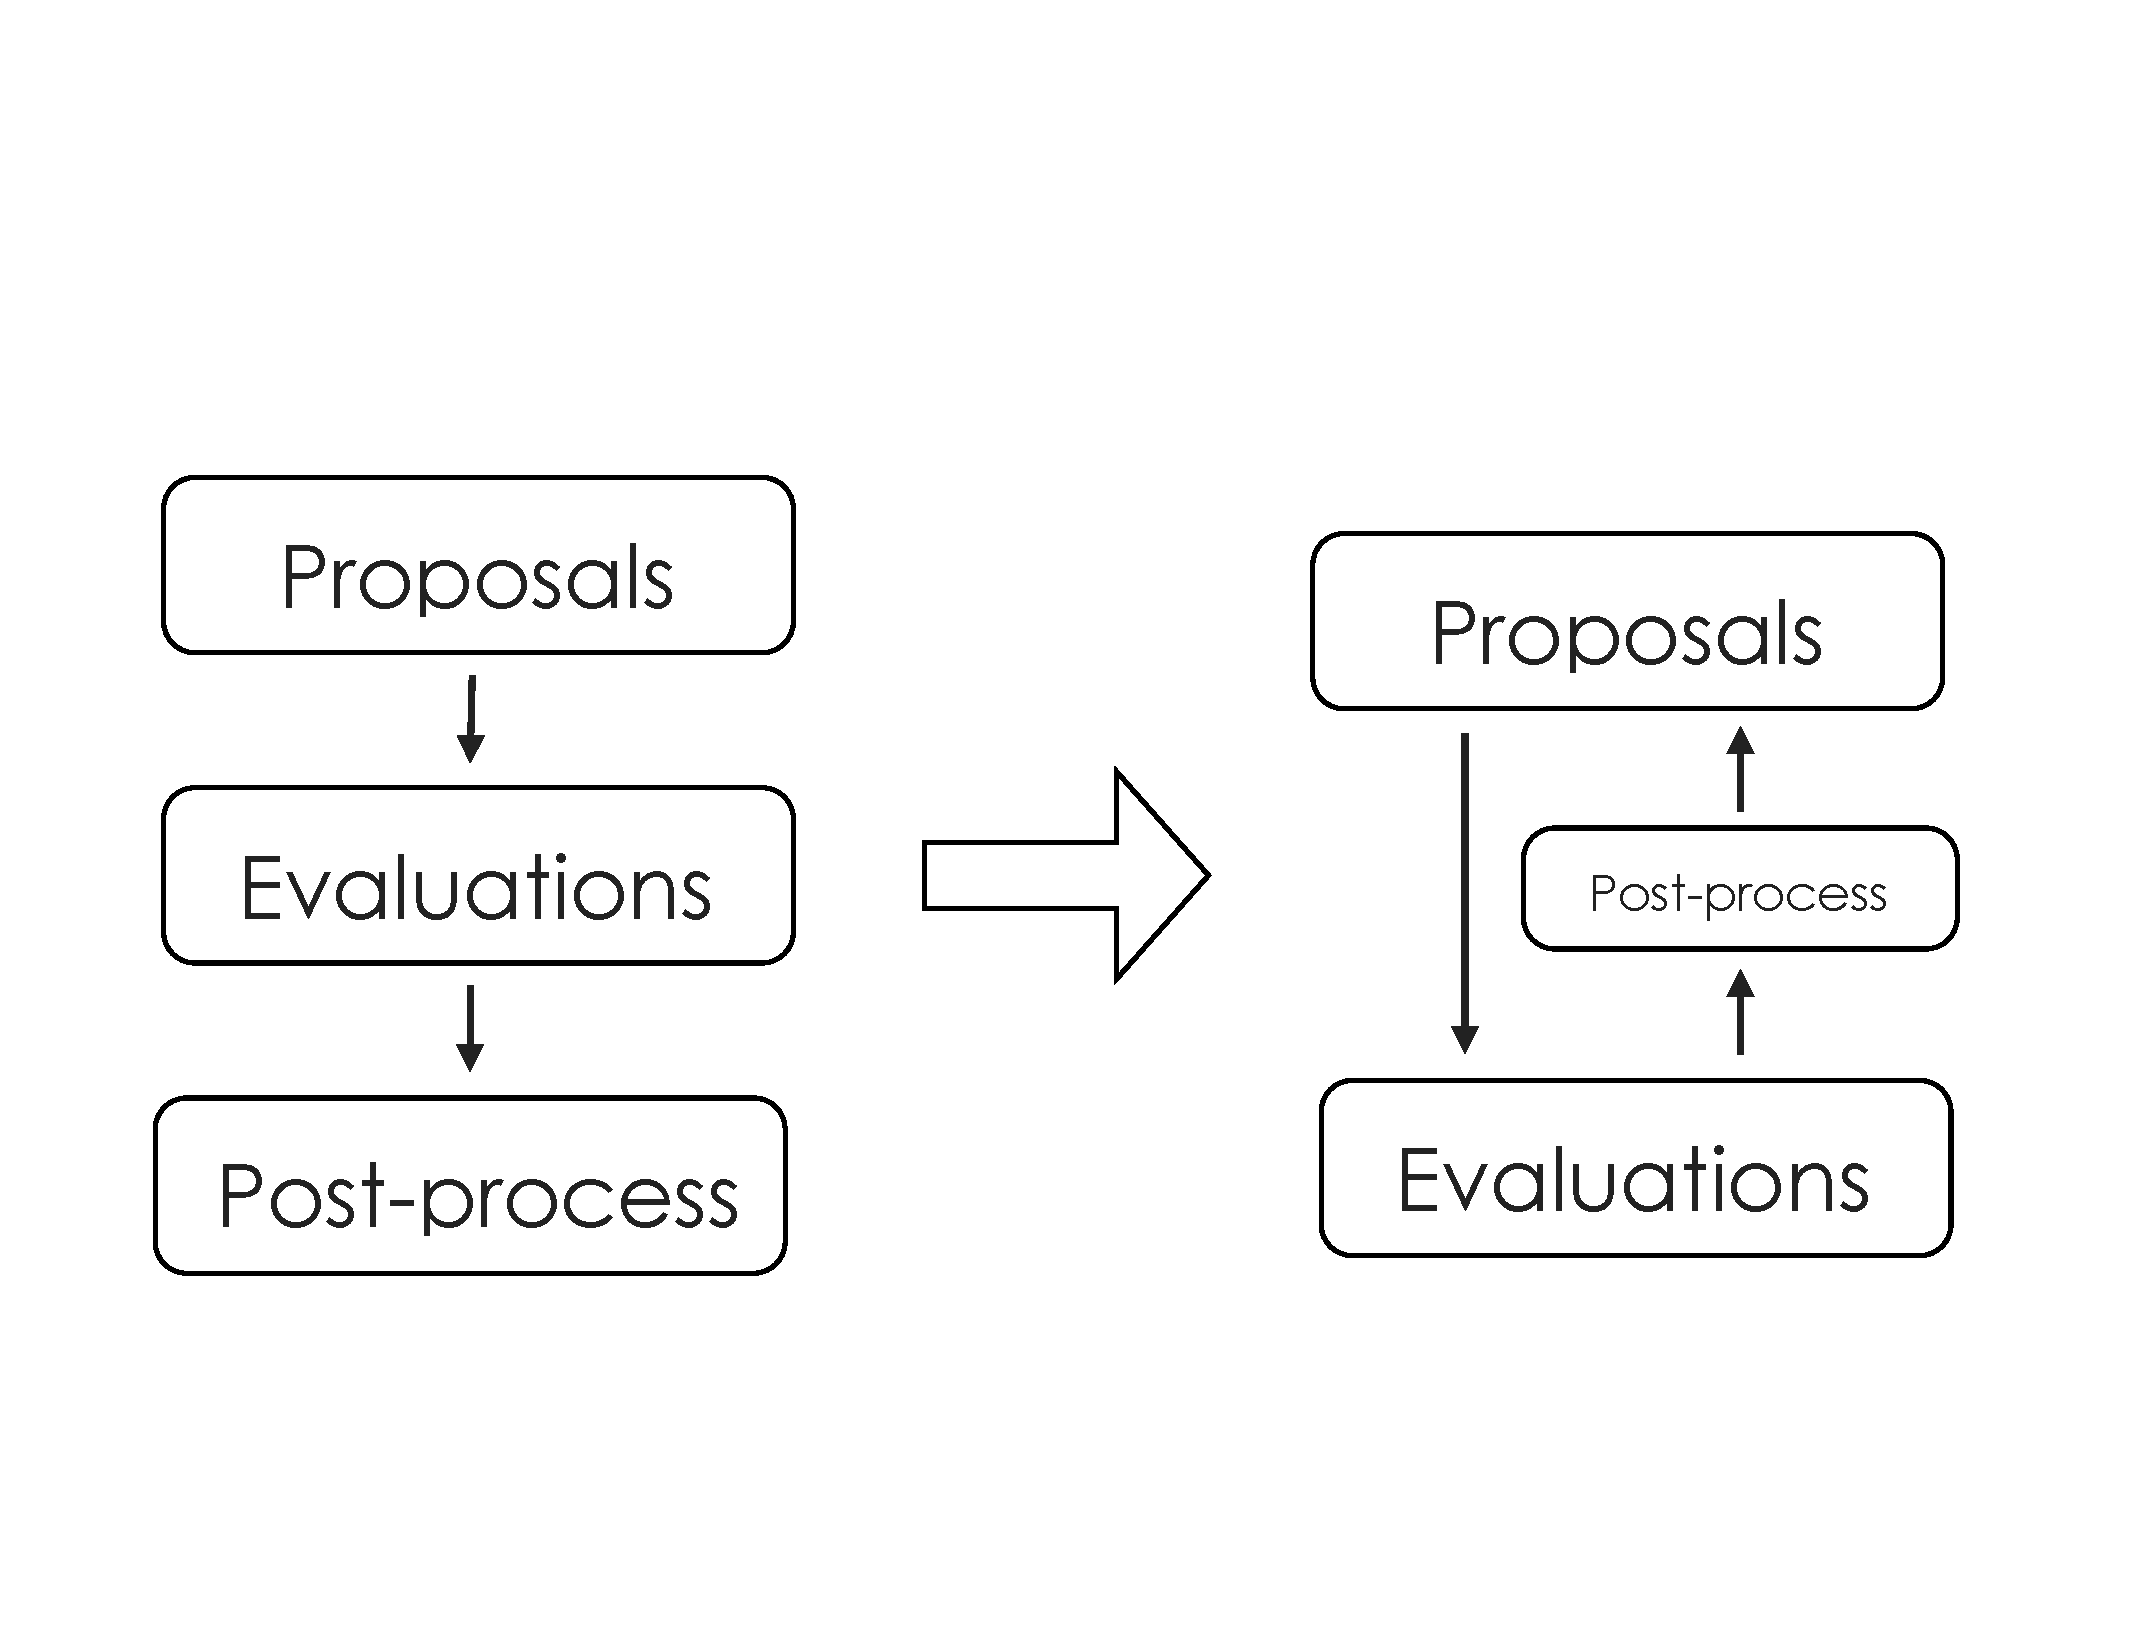
\includegraphics[width=0.9\linewidth]{../figures/architecture_concept.pdf}
  \label{fig:architecture_concept}
\end{figure}

Taking a grander view, most current detection systems can be conceptualized as having three parts, as visualized in~\autoref{fig:architecture_concept}.

The region proposal is usually done exhaustively over the image space, and doing so in an efficient order has not received much attention in the literature.
Using jump windows as region proposals is one common idea~\cite{Chum2007b,Vijayanarasimhan2011}.
For local features, a bounded search over the space of all possible windows works well (especially for single-object detection)~\cite{Lampert2008b}.
The method requires derivation of bounds, which have not yet been developed for HOG-based detectors, limiting the method's usefulness in state-of-the-art systems.
Similar ideas have been formulated in a decision theoretic way~\cite{Sznitman2010}.

Region proposal through segmentation is another common idea~\cite{Russakovsky2010}.
\note{more here.}

Another idea is to use a class-independent measure of ``objectness'' to reject much of the hypothesis space before running any class-specific detectors~\cite{Alexe2010,Endres2010}.
However, the latter approach has not been shown to be actually faster than exhaustive evaluation, either because the proposal step becomes too expensive~\cite{Endres2010}, or because the system was not coded efficiently~\cite{Alexe2010}.

In search of efficient detectors, the general ``cascade'' idea of breaking up the evaluation of an image region into thresholded steps has been applied to current state-of-the-art systems~\cite{Vedaldi2009, Felzenszwalb2010a}.
In the case of the Multiple-Kernel Detector~\cite{Vedaldi2009}, the cascade is necessary to keep detection of a single class to the order of a minute per image.
In the case of the Deformable Parts Model~\cite{Felzenszwalb2010a}, the cascade speeds up detection from several seconds to under a second per class, with little loss in accuracy.

Evaluation of regions involves feature computation, which is a time consuming step.
Efficient feature computation for HOG-based detectors has been explored in~\cite{Dollar2010}.
Another idea is coarse-to-fine model evaluation.
A recent work applies coarse-to-fine evaluation and adds a feedback arrow from post-processing to proposals, obtaining an order of magnitude speedup in the deformable part models framework while losing some accuracy~\cite{Pedersoli2011}.

Other systems that add feedback arrows to the conceptual diagram in~\autoref{fig:architecture_concept} are often inspired by biological vision and sequential decision process ideas~\cite{Butko2009,Vogel2008,Paletta2005}.
\note{more}

A close relative to this idea is inspired by the problem of tracking objects.
A recent paper draws an interesting feedback arrow from Evaluations to Proposals by using iterative sampling of a hypothesized mixture of Gaussians to find multiple objects in the image~\cite{Gualdi2010}.

Anytime performance in vision systems is a surprisingly little-explored idea.
A pioneering recent paper picks features with maximum value of information in a Hough-voting framework, and explicitly evaluates itself with regard to time \cite{Vijayanarasimhan2010}.

Multi-class detection has its own line of work, focusing largely on detection time sublinear in the number of classes through sharing features~\cite{Torralba2007,Fan2005,Razavi2011}.
An interesting reinforcement learning approach in a cascade framework is taken in~\cite{Isukapalli2006}.
\note{more}

A recent post-processing extension to detection systems uses structured prediction to incorporate multi-class context as a principled replacement for the common step of non-maximum suppression~\cite{Desai2009}.
This work aims to tie up a couple of loose threads of object detection: 1) joint multi-class detection, with the mutual exclusion and contextual effects it entails; 2) the hack of non-maximum suppression of single-class detections.

Context has a long history in vision.
One source of context is the scene or non-detector cues; for the PASCAL VOC, these are quantitatively considered in~\cite{Divvala2009}.
Another source is inter-object context, used for detection in a random field setting in~\cite{Torralba2004}.
\note{more}

Brief review of attentional modeling work~\cite{Itti2001a,Chikkerur2010,Judd2009}.
The concept of saliency has been used for object classification \cite{Kanan2010}.

\note{todo: active recognition~\cite{Denzler2002,Andreopoulos2009}.}

The two papers closest to our contribution are principled multi-class structured prediction~\cite{Desai2009} and the detection under bounded resources work~\cite{Vijayanarasimhan2010}.
We significantly extend the first work, which assumes that all classes have been evaluated at all regions, to the online case of picking regions and classes to evaluate.
We are guided by the same motivation of Anytime performance as the second work, but in a significantly more powerful detection regime.
Although we rely on the commonly used deformable parts model detector, our method can use any feature extraction and classification method.